%!TEX TS-program = xelatex

\documentclass[12pt]{article}

\usepackage{tgtermes}

% Table
\usepackage{booktabs}
\usepackage[flushleft]{threeparttable}

% Font
\usepackage[T1]{fontenc} % Font encoding
\usepackage{lmodern,microtype} % Typeface

% Math
\usepackage{amsmath,amsthm,amssymb,amsfonts} % AMS math
\usepackage{dsfont,mathrsfs,ushort} % Math style
\usepackage{mathtools}

% Style
\usepackage{titlesec,titling} % Section titles
\usepackage[nohead]{geometry} % Page & margins
\usepackage{setspace} % Spacing
\usepackage{enumitem,booktabs} % Tables & lists

% References
%\usepackage[comma]{natbib} % Unused options: [sort] [sort&compress] [merge]
\usepackage[style=authoryear]{biblatex} 
\addbibresource{citation.bib}
\usepackage{thmtools,thm-restate}

% Addons
\usepackage{pstricks} % Figures
\usepackage{sgamevar} % Strategic form games

%example-continued
\usepackage{thmtools}
\declaretheorem[style=definition]{example}
\renewcommand\thmcontinues[1]{Continued}

% Institute
\usepackage[affil-it]{authblk}


% Hyperlinks
\usepackage{hyperref}

% suppress the black rectangle 
\overfullrule=0pt

\usepackage[splitrule]{footmisc} %% The splitrule option draws a full width rule above the continued part of the footnote as a visual cue to readers.
\interfootnotelinepenalty=10000 %% Completely prevent breaking of footnotes


\newtheorem{thm}{Theorem}
\newtheorem{defn}{Definition}
\newtheorem{assp}{Assumption}
\newtheorem{eg}{Example}
\newtheorem{lem}{Lemma}
\newtheorem{cor}{Corollary}
\newtheorem{rmk}{Remark}

\DeclareMathOperator*{\argmax}{arg\,max}
\DeclareMathOperator*{\argmin}{arg\,min}
\newcommand{\Indc}{\mathbb{I}}
\newcommand{\md}{\mathrm{d}}
\newcommand{\Ep}{\mathbb{E}}
\newcommand{ \littleop}{o_p}
\DeclarePairedDelimiter{\norm}{\lVert}{\rVert}

%%%%%%%%%%%%%%%%%%%%%%%%%%%%%%%%%%%% Frontmatter
\title{\bfseries\Large Sensitivity Analysis for Estimation of Long-Term Treatment Effects \vspace*{-1ex}}
\author{\large\textit{Han Xu} \\
	\large \textup{Pennsylvania State University}\\\textup{hfx5023@psu.edu}}

\date{\today}


%%%%%%%%%%%%%%%%%%%%%%%%%%%%%% Style & Structure
% Hyperlinks
\hypersetup{
	colorlinks=true,
	linkcolor=blue,
	filecolor=magenta,      
	urlcolor=cyan,
	pdftitle={sensitivity},
	pdfpagemode=FullScreen,
}

% Titles
\titleformat{\section}[block]{\centering\large\bfseries}{\thesection.}{0.5em}{}
\titleformat{\subsection}[block]{\flushleft\bfseries}{\thesubsection.}{0.5em}{}
\titleformat{\subsubsection}[runin]{\normalsize\itshape}{\bfseries\thesubsubsection.}{0.5em}{}[.--\:]
\renewcommand{\thesubsubsection}{\arabic{section}.\arabic{subsection}.\alph{subsubsection}}
\titlespacing{\section}{0ex}{6ex}{3ex}
\titlespacing{\subsection}{0in}{3ex}{1.5ex}
\titlespacing{\subsubsection}{0mm}{2ex}{0.5em}
\renewcommand{\linespread}[1]{\setstretch{1}}
\linespread{2}
\begin{document}
	
	\maketitle
	
	%\begin{abstract}
	%\textcite{athey2020combining} proposed a data combination approach to identify the effect of treatment on long term outcome, where they rely on unconfoundedness in an experimental sample and latent unconfoundedness in an observational sample. This paper shows how to construct bounds for the effect of treatment on long-term outcome when we only have partial (latent) unconfoundedness, using technique in \textcite{yadlowsky2018bounds}, which is based on a likelihood ratio restriction. Estimators for bounds and accompanied inference procedure are also shown. Finally, I provide examples involving both simulated and real data to illustrate the accuracy of confidence interval and its practical significance.
	%\end{abstract}

    \section{INTRODUCTION}
    
    Estimation of the long-term effects of a policy/treatment is crucial since it lays the foundation for many real-world policy decisions, such as class size adjustment and poverty alleviation. One challenge in estimation of the long-term effect is that it's often hard to use a randomized experiment to study the effect directly due to the delay of response. Recently, \textcite{athey2020combining} show that a combination of short-term experimental sample and long-term observational sample can help achieve identification (and also estimation of) long-term effects. In the experimental data, the researcher observes the randomized treatment and the short-term outcome($S$). In the observational data, the researcher observes the confounded treatment, short-term outcome($S$), and the long-term outcome($Y$). The key assumptions for identifications are as follows: treatment in the experimental sample is unconfounded, treatment in the observational sample is latent-unconfounded, and the two samples are "comparable"--which is often referred to as external validity in the literature.
	
	However, in real-world data, the above assumptions could be violated. Altough the unconfoundedness assumption in the experimental sample can be ensured if we use randomization scheme, the other two suffer from a variety of problems. For example, the latent unconfoundedness assumption can be shown to fail when a dimension restriction is violated: there are more independent confounding factors affecting the treatment assignment process than independent short-term outcome variables. The sample comparability condition, on the other hand, could fail as a result of selection bias: the experimental sample is not representative of the target distribution, even after we control for covariates. Moreover, it is widely known that without additional restrictions on the model, these assumptions are non-refutable. Namely, the data alone cannot tell us whether it is true. 
	
	Nonetheless, researchers interested in estimation of long-term treatment effects may want to assess how sensitive their results are to failures of these assumptions. A large literature on sensitivity analysis has developed to answer this question. Recent work by \textcite{masten2018identification, yadlowsky2018bounds, kallus2018confounding} each develop a nonparametric relaxation of the unconfoundedness assumption, which does not rely on auxiliary functional form or parametric distribution assumptions\footnote{Until recently, most approaches rely on strong auxiliary assumptions such as linearity of model or normality of the confounding factor, which can be undesirable because these auxiliary assumptions themselves is not needed for identification. }. Usually, the sensitivity analysis will produce a set of bounds corresponding to different choice of sensitivity parameters, and therefore allow researchers to evaluate how robust their results are to slight or severe violation of assumptions. However, most existing sensitivity analysis do not accommodate relaxation of multiple assumptions, and therefore cannot be directly used to assess the sensitivity of results to the above collection of assumptions. The propogation of sensitivity is new to the analysis. Take the estimation of long-term treatment effects as an example: we might interested in knowing how sensitive the results are to the relaxation of the latent unconfoundedness assumption if we've already relaxed the sample comparability assumption.
	
	In this paper, I provide a method of sensitivity analysis for the data-combination scenario in the work of \textcite{athey2020combining}. Specifically, I apply the identification results of \textcite{yadlowsky2018bounds}, who uses likelihood-ratio restrictions to measure the relaxation of unconfoundedness-type assumptions. The likelihood-ratio restriction is directly interpretable: it controls the dependency of odds-ratio on unmeasured confounding factors. For each assumption, I introduce a sensitivity parameter to measure how severely it is violated. Extending the single-sample case, we derive bounds for quantities of interest, such as average treatment effect (ATE) on the long-term outcome. Regarding the propagation of sensitivity, we'll see that the relaxation of one assumption is complementary to the relaxation of the other in terms of bounding the target parameter.
	
	%Many interesting problems arise as one think about assessing sensitivity to multiple assumptions.  Another problem concerns the interpretation on sharpness of bounds. When there is only one assumption to be relaxed, many existing methods provide bounds that are sharp, i.e., that's attainable by some DGP that's consistent with the choice of sensitivity parameters. However, when there are multiple assumptions to be relaxed, the sharpness of bounds is more subtle.
	
	Based on the identification result, I also study the estimation and inference of bounds in the data combination context. I translate the defining equations of bounds into a set of moment conditions and propose a Method of Moment(MM) estimator. When $S$ takes only discrete value, the asymptotic property of this MM estimator is derived. An application of delta method then gives the asymptotic distribution of bounds on $\tau$. The case where $S$ can take a continuum of values is more complicated, and is not covered in this version. With the estimation procedure, empirical researchers interested in using ACI's method to estimate long-term treatment effects can use these estimated identified sets (and accompanying confidence interval) to examine how sensitive their parameter estimates are to deviations from the baseline assumption latent unconfoundedness and external validity. Finally, I provide an example involving simulate data to illustrate the accuracy of estimation and inference procedure and its practical significance. 
	

	\medskip
	\textbf{Related Literature} In the rest of this section, I review the related literature.
	This paper connects with the work by \textcite{athey2020combining}, who pioneer the use of latent unconfoundedness assumption. It also contributes to a growing literature on sensitivity analysis, see, e.g., \textcite{masten2018identification, yadlowsky2018bounds}. The sensitivity analysis of sample comparability is related to the sample comparability literature. 

	\section{MODEL, ASSUMPTIONS, AND INTERPRETATION}
	I study the problem of identifying long-term treatment effects as in \textcite{athey2020combining}(For convenience, I refer to the paper as ACI henceforth). In this section
I set up the notation and some maintained assumptions. I review parameters of
interest and state the key assumption which point identifies them, which are given in ACI. I discuss how I relax those assumptions. Identified sets under these relaxations are derived in Section 3. I conclude this section by providing an interpretation of the deviations from baseline assumptions.
	
	
	\subsection{Notation}
	There are two available samples. Following \textcite{athey2020combining}, I will call them the experimental sample and the observational sample. Here the name "experimental sample" should not be taken literal since it could be generated by non-randomized assignment mechanism. Rather, it's just a label on the sample. We use $G$ to denote sample(group), $G=E$ for experimental and $G=O$ for observational, There is a single treatment that we are interested in. The treatment effects model follows the “potential outcomes” approach of \textcite{rubin1974estimating}. Instead of a single treatment variable as in most literature, we use two treatment variables to indicate the potentially different nature of the assignment mechanism. The treatment variable in the experimental sample is denoted as $T$, and the treatment variable in the observational sample is denoted as $D$\footnote{This is mainly for ease of demonstration. One can use the same variable accompanied $G = E$ or $G = O$ to differentiate the two cases. I just find using two variables more handy sometimes.}. There are two different sets of potential outcomes. The secondary (short-term) outcome, denoted by $S(d) \in \mathbb{R}$ for $d\in \{0,1\}$, are auxiliary for identification.  The primary (long-term) outcome is denoted as $Y(d) \in R$. Here $Y = Y(1)D + Y(0)(1-D)$ and $S = S(1)D + S(0)(1 - D)$. 

	\subsection{Review of Identification Assumptions in ACI(2020)}
	The goal of \textcite{athey2020combining} is to identify $\Ep[Y(1) - Y(0) \mid G = O]$, the ATE in the observational sample. To achieve identification, they make the following assumptions\footnote{In their work, they also include a covariate vector $X$, which we will omit here.}.
	\begin{assp}[Unconfoundedness in $G = E$]\label{a1}
		For $t \in\{0,1\}$,
		$$T_i \perp S_i(t) | G_i = E\footnote{Here I am working with "weak" unconfoundedness since I do not assume the joint independence of $S(0), S(1)$ and $D$. Unless mentioned, all unconfoundedness is weak unconfoundedness in this paper. For a discussion, see \textcite{imbens2000role}.}$$
	\end{assp}
		
	\begin{assp}[Sample comparability of $G = E$ and $G = O$]\label{a2}
		
		\begin{equation*}
		G_{i} \perp\left(Y_{i}(0), Y_{i}(1), S_{i}(0), S_{i}(1)\right)\footnote{In \textcite{athey2020combining}, they work with the following one called conditional sample comparability with $X_i$ being some additional covariates:
			$$
			G_{i} \perp\left(Y_{i}(0), Y_{i}(1), S_{i}(0), S_{i}(1)\right) \mid X_{i}
			$$It can be seen that it's just a conditional version of the current one. To simplify analysis, I will use the direct comparability throughout.}
		\end{equation*}
	\end{assp}
	
	\begin{assp}[Latent Unconfoundedness]\label{a3}
		For $d \in\{0,1\}$,
		$$
		D_{i} \perp Y_{i}(d) \mid S_i(d), G_{i}=\mathrm{O}
		$$
	\end{assp}
	% Intuitively, what it says is that the effects of the treatment on the short-term and long-term outcomes have the same set of unobserved confounding variables\footnote{ \textcite{athey2020combining} compare this assumption to a control function in a non-parametric instrumental variables setting. They show that, for exact identification, the unobserved confounder in the observational sample cannot have a dimension higher than that of the secondary outcome. It's understood as a rank restriction or dimension restriction.}.
	
	ACI show that we can identify $\tau = \Ep[Y(1) - Y(0) \mid G = O]$ given the above assumptions. For completeness, I include a proof of the result below, which inspires the derivation of bounds when the assumptions are relaxed.
	\begin{restatable}{thm}{identification}{}\label{iden}
			Under A1-A3, $\mathbb{E}[Y(1) \mid G = O]$ and $\mathbb{E}[Y(0) \mid G = O]$ are identified.
	\end{restatable}
	
	\begin{proof}
		I focus on identification of $\Ep[Y(1) \mid G = O]$, since the counterpart for $\Ep[Y(0) \mid G = O]$ is achieved similarly. 
		
		By law of iterated expectation, $\mathbb{E}[Y_i(1) \mid G = O] = \mathbb{E}[Y_i(1) \mid D_i = 0, G = O] P(D_i = 0 \mid G = O) + \mathbb{E}[Y_i(1) \mid D_i = 1, \mid G = O] P(D_i = 1, \mid G = O)$. The only non-directly-identified part is $E[Y_i(1) \mid D_i = 0, \mid G = O]$. This is equal to 
		\begin{align*}
		& \mathbb{E}[\mathbb{E}[Y_i(1) \mid S_i(1), D_i = 0, G = O] \mid D_i = 0, G = O] \\
		& = \int\mathbb{E}[Y_i(1) \mid S_i(1) = s, D_i = 0, G = O]  dP_{S(1) \mid D = 0, G = O}(s)\\
		& = \int \mathbb{E}[Y_i(1) \mid S_i(1) = s, D_i = 1, G = O] dP_{S(1) \mid D = 0, G = O}(s) \\
		& = \int \mathbb{E}[Y_i \mid S_i = s, D_i = 1, G_i = O] dP_{S(1) \mid D = 0, G = O}(s)
		\end{align*}
		We need the experimental data to identify $P_{S(1) \mid D= 0, G = O}(s)$. This is possible since
		$$
		P_{S(1) \mid G = O}(s) = P_{S(1) \mid D= 0, G = O}(s) P(D = 0 \mid G = O) +  P_{S(1) \mid D=1, G = O}(s) P(D = 1 \mid G = O)
		$$
		and $P_{S(1) \mid G = O}, P_{S(1) \mid D=1, G = O}(s)$ are identified from the experimental and observational data separately. Indeed, $P_{S(1) \mid G = O}(s) = P_{S(1) \mid G = E}(s) = P_{S(1) \mid D = 1, G = E}(s)$ by unconfoundedness and $P_{S(1) \mid D=1, G = O}(s) = P_{S \mid D = 1, G = O}(s)$, which is identified from the observational sample.
	\end{proof}
	
	In the proof above, the assumptions are essentially used to perform changes of measure, or changes of the conditioning sets. More specifically, A\ref{a1} is used to show $P_{S(1) \mid G = E}(s) = P_{S(1) \mid D = 1, G= E}(s)$; A\ref{a2} is used to show that $P_{S(1) \mid G = E}(s) = P_{S(1) \mid G = O}(s)$; A\ref{a3} is used to show $ \mathbb{E}[Y_i(1) \mid S_i(1) = s, D_i = 1, G = O] = \mathbb{E}[Y_i(1) \mid S_i(1) = s, D_i = 0, G = O]$. Naturally, one might see that by relaxing these assumptions, the equality breaks and point identification of $\Ep[Y(1) \mid G = O]$ is no longer available.
	
	In \textcite{athey2020combining}, the authors mention that it's often easy to ensure that A\ref{a1}(unconfoundedness in the experimental sample) is satisfied, since the researcher can often use randomization in assignment of treatment. However, the validity of A\ref{a2} and A\ref{a3} are not guaranteed.
	
	\subsection{Restriction on Likelihood Ratio}
	Let $K$ and $H$ be real numbers larger than or equal to 1. The following definitions characterize relaxations of latent-unconfoundedness and sample comparability in respect.
	
	\begin{defn}[$K-$(latent)-confoundedness] Let $L^d(y,s) = \frac{\mathrm{d} P(Y_i(d) = y \mid S_i(d) = s, D_i =1-d, G_i = O)}{\mathrm{d} P(Y_i(d) = y \mid S_i(d) = s, D_i = d, G_i = O)}$. Suppose $$L^d(y,s) \leq K L^d(y',s) \quad \forall y,y',s \text{ and } d\in\{0,1\}.$$ Then the distribution of primitives satisfy $K$-(latent)-confoundedness. In what follows, I will just refer to it as $K$-confoundedness. It relaxes the latent-unconfoundedness assumption in the observational sample.
	\end{defn}
	
	\begin{defn}[$H$-comparability]
	 Let $L^t(s) = \frac{\mathrm{d} P(S_i(t) = s \mid G_i = O)}{\mathrm{d} P(S_i(t) = s \mid G_i = E)}$. Suppose $$L^t(s) \leq H L^t(s') \quad \forall s,s' \text{ and } t \in \{0,1\}.$$ Then the distribution of primitives satisfy $H$-external-validity. It relaxes the sample comparability assumption.
	\end{defn}

	When $K$ and $H$ are equal to 1, we are back in the identified case. The restrictions are direct consequences of a change of measure, since, for example, $$\Ep[Y(1) \mid S(1) = s, D = 0, G = O] = \Ep[L^1(Y(1),s) Y(1) \mid S(1) = s, D = 1, G = O].$$ In fact, the likelihood ratio restriction is equivalent to a functional form restriction on the log odds ratio. 
	The following result adapted from \textcite{yadlowsky2018bounds} shows the case for $K$-confoundedness.
	
	\begin{restatable}{lem}{confound}
		\label{confound}
		Suppose $$Y(1) \perp D \mid S(1), U, G = O.$$
		The following three conditions are equivalent:
		\begin{enumerate}[label=(\alph*)]
			\item The log odds ratio has the following form $$\log \left(\frac{P(D=1 \mid S(1) = s, U=u, G = O)}{P(D=0 \mid S(1)=s, U=u, G = O)}\right)=\kappa(s)+\log (K) b(u)$$
			where $u$ stands for the unmeasured confounding variable, $b(u)$ is some real-valued function that takes value in $[0,1]$.
			\item $\forall u, u',$ $$\frac{P(D=1 \mid S(1) = s, U=u, G =O)}{P(D=0 \mid S(1)=s, U=u, G = O)} \times\frac{P(D=0 \mid S(1) = s, U=u', G =O)}{P(D=1 \mid S(1)=s, U=u', G = O)} \leq K.$$
			\item For fixed $s$, let $L^1(y,s) = \frac{\mathrm{d} P(Y_i(1) = y \mid S_i(1) = s, D_i = 0, G = O)}{\mathrm{d} P(Y_i(1) = y \mid S_i(1) = s, D_i = 1, G = O)}$. Then $L^1(y,s) \leq K L^1(y',s) \quad \forall y,y'$.
		\end{enumerate}
	\end{restatable}
	\begin{proof}
	    The proof is essentially the same as those given in \textcite{rosenbaum2002overt}, if we treat $S(1)$ as a covariate variable.
	    
		Equivalence of $(a)$ and $(b)$ is given in \textcite{rosenbaum2002overt}. Equivalence of $(b) \text{ and } (c)$ is given in \textcite{yadlowsky2018bounds}.
	\end{proof}
	
	Similarly, if we interpret $G_i$ as a "treatment" assignment, and $S_i(d)$ as the target outcome, we can provide a set of equivalent conditions for $H-$comparability.
	
	\section{IDENTIFICATION}
	
	In this section, I study (partial) identification of long-term treatment effects when A\ref{a2} or A\ref{a3} are not satisfied. To do so, I start by introducing a lemma which is useful for bounding the mean of unavailable counterfactual outcome. I then apply these results to obtain sharp bounds on $\Ep[Y(1) \mid G = O]$. The analysis for bounds on $\Ep[Y(0) \mid G = O]$ is similar and is omitted.
	
	\subsection{Bounds}
	
	The following lemma extends Lemma 2 in \textcite{yadlowsky2018bounds}, and is very useful for establishing the bounds. The original proof is a special case of the current one when $W(1)$ is scalar valued and $f$ is the identity map.
	
	\begin{restatable}{lem}{duality}
		\label{duality}
		Consider a potential outcome framework where the treatment variable is $D_i$ and the potential outcome is $W_i(1)$. Let $f:R^m \to R$ be a known $\sigma_{W(1)}$-measurable function and $$\mathbb{E}[\|f(W(1))\| \mid D=1] < \infty.$$
		Let $L(w) = \frac{\mathrm{d} P(W_i(1) = w \mid D_i = 0)}{\mathrm{d} P(W_i(1) = w \mid D_i = 1)}$.
		Consider the problem \begin{equation*}
		\begin{array}{ll}
		\inf _{L(w)} & \mathbb{E}[L(W(1))f(W(1)) \mid D=1] \\
		\text { s.t. } & \mathbb{E}[L(W(1)) \mid D=1]=1 \\
		& L(w) \geq 0, L(w) \leq B L(\tilde{w}) \text { for almomst every } y, \tilde{y} \in \mathbb{R}.
		\end{array}
		\end{equation*}
		The solution to it is identical to 
		\begin{equation*}
		\begin{array}{ll}
		\sup _{\mu} & \inf _{L(w)} \quad \mathbb{E}[(f(W(1))-\mu) L(W(1)) \mid D=1]+\mu \\
		\text { s.t. } &\quad  L(w) \geq 0, L(w) \leq B L(\tilde{w}) \text { for almomst every } w, \tilde{w} \in \mathbb{R}.
		\end{array}
		\end{equation*}
		which is further equal to
		\begin{equation*}
		\begin{array}{ll}
		\sup _{\mu} & \mu \\
		& \text { s.t. }  \mathbb{E}\left[(f(W(1))-\mu)_{+}-B(f(W(1))-\mu)_{-} \mid D=1\right] \geq 0.
		\end{array}
		\end{equation*}
		Moreover, the above inequality is actually an equality. The bound given here is sharp: there exists some $L$ such that the lower bound is attained.
	\end{restatable} 
	
	\begin{proof}
		See appendix. Also, there is a counterpart for \begin{equation*}
		\begin{array}{ll}
		\sup _{L(w)} & \mathbb{E}[L(W(1))f(W(1)) \mid D=1] \\
		\text { s.t. } & \mathbb{E}[L(W(1)) \mid D=1]=1 \\
		& L(w) \geq 0, L(w) \leq B L(\tilde{w}) \text { for almost every } y, \tilde{y} \in \mathbb{R}.
		\end{array}
		\end{equation*}
		For this problem, the solution is identical to \begin{equation*}
		\begin{array}{ll}
		\inf _{\mu} & \mu \\
		& \text { s.t. }  \mathbb{E}\left[(\mu-f(W(1)))_{+}-B(\mu-f(W(1)))_{-} \mid D=1\right] \geq 0.
		\end{array}
		\end{equation*}
		
		To prove it, just replace $f$ by $-f$ and use the above lemma. Therefore the lemma also gives us an expression for the upper bound.
	\end{proof}
	
	Lemma \ref{duality} relates the restriction on the likelihood profile to bounds on mean of counterfactual outcome. When $B = 1$, the restriction is strong since it requires that the likelihood for observing certain $w$ to be equal for treatment status. In this case, $\mathbb{E}\left[(f(W(1))-\mu)_{+}-B(f(W(1))-\mu)_{-} \mid D=1\right] = \mathbb{E}\left[(f(W(1))-\mu) \mid D=1\right] = 0$, so we are back in the case where $\Ep[f(W(1))]$ can be identified. When $B$ is larger than 1, the restriction is relaxed, and the lower bound is smaller than $\Ep[f(W) \mid D = 1)]$. Also, it's readily seen as $B$ increase, the lower bound will get looser, so the bound on $\Ep[f(W(1)) \mid D = 0]$ will be monotonic in the sensitivity parameter $B$ here. 
	
	With these tools, we can establish bounds for $\Ep[Y(1)] \mid D = 0, G = O]$, which then allow us to bound $\Ep[Y(1)] \mid G = O]$. Take the lower bound of $\Ep[Y(1) \mid D= 1, G = O]$ as an example, we have the following theorem:
	\begin{restatable}[Bounds on $\Ep(Y(1) \mid D = 0, G = O)$]{thm}{lb}\label{thm:thm2}
		We maintain the assumption of randomization  in the experimental sample throughout.
		\begin{enumerate}[label=(\alph*)]
			\item Under $K$-confoundedness and external-validity, we have the following lower bound for $\Ep[Y(1) \mid D = 0, G = O]$:
			$$\mu^-_1 = \int \theta_1(s) \mathrm{d} P_{S(1) | D = 0, G = O}(s)$$ where 
			\begin{equation}\label{eq:eq1}
			\begin{array}{ll}
			\theta_1(s) \coloneqq & \sup _{\mu}  \mu \\
			& \text { s.t. }  \mathbb{E}\left[(Y(1)-\mu)_{+}-K(Y(1)-\mu)_{-} \mid S(1)=s, D=1, G = O\right] \geq 0,
			\end{array}
			\end{equation}
			and 
			\begin{equation}\label{eq:eq2}
			P_{S(1) \mid D = 0, G = O} (\cdot) = \frac{P_{S \mid D = 1, G = E}(\cdot) - P_{S \mid D = 1, G = O} (\cdot) P(D = 1 \mid G = O) }{P(D = 0 \mid G = O)}.    
			\end{equation}
			
			
			\item Under $K-$latent-unconfoundedness and H-comparability, we have the following lower bound for $\Ep[Y(1) \mid D = 0]$:
			
			\begin{equation}\label{eq:eq3}
			\begin{array}{ll}
			\mu_1^- =  \frac{\zeta_1^- - \Ep[\theta_1(S) \mid D=1, G=O] P(D=1\mid G=O)}{P(D = 0 \mid G = O)}
			\end{array}
			\end{equation}
			where 
			\begin{equation}\label{eq:eq4}
			\begin{array}{ll}
			\zeta_1^- \coloneqq & \sup _{\mu}  \mu \\
			& \text { s.t. }  \mathbb{E}\left[(\theta_1(S)-\mu)_{+}-H(\theta_1(S))-\mu)_{-} \mid D=1, G = E\right] \geq 0,
			\end{array}
			\end{equation}
			
		\end{enumerate}
	\end{restatable}
	
	Theorem \ref{thm:thm2} shows the how the sensitivity is propagated through relaxation of multiple assumptions. Note that in case (a), only the latent-unconfoundedness assumption is relaxed, and the lower bound for $\Ep[Y(1) \mid D = 0, G =O]$ is an conditional expectation of the lower bound $\theta_1(s)$; in (b), the sensitivity margin introduced by relaxing the sample comparability assumption is also taken into account, which complements the lower bound $\theta_1(s)$. 
	
	A similar upper bound for $\Ep[Y(0) \mid D = 1, G= O]$ is available, by using the upper bound counterpart of lemma \ref{duality}. The result is given below.
	\begin{cor}
			Under $K$-confoundedness and $H-$comparability, we have the following identified upper bound for $\Ep[Y(0) \mid D = 1, G= O]$:
			$$
			\mu^+_0 =\frac{\zeta_0^+ - \Ep[\theta_0(S(0)) | D = 0, G = O] P(D = 0 \mid G = O)}{P(D = 1 \mid G = O)}
			$$
			where 
			\begin{equation}\label{eq:eq5}
			\begin{array}{ll}
			\theta_0(s) \coloneqq & \inf _{\mu}  \mu \\
			& \text { s.t. }  \mathbb{E}\left[(\mu - Y(0))_+ - K (\mu - Y(0))_- \mid S(0) = s, D = 0, G = O \right] \geq 0.
			\end{array}
			\end{equation}
			and
			\begin{equation}\label{eq:eq6}
			\begin{array}{ll}
			\zeta_0^+ \coloneqq & \inf _{\nu}  \nu \\
			& \text { s.t. }  \mathbb{E}\left[(-\theta_0(S)+\nu)_{+}-H(-\theta_1(S)+\nu)_{-} \mid D=0, G = E\right] \geq 0.
			\end{array}
			\end{equation}
	\end{cor}
	
	Using these bounds we obtain a lower bound for $\tau = \Ep[Y(1) - Y(0) \mid G = O]$:
	\begin{eqnarray*}
		\tau^-  & = & \left[\Ep[Y(1) \mid D = 1]P(D = 1) + \mu_1^-  P(D = 0)\right] - \\
		 & & \quad \left[\Ep[Y(0) \mid D = 0]P(D = 0) + \mu_0^+ P(D = 1)\right].
	\end{eqnarray*}
	
	It's also direct to extend these argument to get an upper bound for $\tau$. To avoid repetitiveness the argument is omitted here.
	
	\subsection{Sharpness of these bounds}
	It's important to remark on the sharpness of these bound. Consider the lower bound for $\Ep[Y(1) \mid D = 0, G = O]$. Under $K-$confoundedness and $H-$comparability, there exist unobservable confounder $U,V$ such that $$\log \left(\frac{P(D=1 \mid S(1) = s, U=u, G = O)}{P(D=0 \mid S(1)=s, U=u, G = O)}\right)=\kappa(s)+\log (K) b(u)$$ with $\norm{b}_{\infty} = 1$, and 
	$$\log \left(\frac{P(G=E \mid V=v)}{P(G=O \mid V=v)}\right)=\kappa'+\log (H) b'(v)$$ with $\norm{b'}_{\infty} = 1$. Note that $\theta_1(s)$ is attained when
	$$L(y,s) = \frac{\mathrm{d} P(Y_i(1) = y \mid S_i(1) = s, D_i =0, G_i = O)}{\mathrm{d} P(Y_i(1) = y \mid S_i(1) = s, D_i = 1, G_i = O)}$$ takes only two values  $\{\frac{K}{K + 1}, \frac{1}{K + 1}\}$ almost surely, and $\zeta_1^-$ is attained when  
	$$L(s) = \frac{\mathrm{d} P(S_i(1) = s \mid G_i = O)}{\mathrm{d} P(S_i(1) = s \mid , G_i = E)}$$
	takes only two values  $\{\frac{H}{H + 1}, \frac{1}{H + 1}\}$ almost surely. It's possible these conditions hold marginally but not jointly\footnote{An extreme case is that $U = V$.}. When $U$ and $V$ are independent, these bounds are sharp.
	
	Therefore, if a DGP satisfies both $K-$confoundedness and $H-$comparability is sharp for each of them, our bounds can still be too loose because of potential dependence of confounders. Compared to existing sharp bounds on the treatment effect, this is undesirable, but that is the price to pay if we do not pursue a parametric approach here.
	
% 	\begin{rmk}[Monotonicity wrt to $K$ or $H$]
% 		It is readily seen that as $K$ or $H$ gets larger, the bound gets looser. Indeed, suppose $K$ gets larger, then in equantion \ref{eq:eq1}:
% 		\begin{equation*}
% 		\begin{array}{ll}
% 			\theta_1(s) \coloneqq & \sup _{\mu}  \mu \\
% 			& \text { s.t. }  \mathbb{E}\left[(f(Y(1))-\mu)_{+}-K(f(Y(1))-\mu)_{-} \mid S(1)=s, D=1\right] \geq 0,
% 		\end{array}
% 		\end{equation*}
% 		an increase in $K$ decreases the value of the left hand side, so it must be compensated by a decrease in $\mu$. Analysis for other cases are similar. Therefore, it is confirmed that increased $K$(or $H$) leads to looser bounds.
% 	\end{rmk}

% 	\begin{rmk}[Weighted Average]
% 		I derive an alternative expression for $\zeta_1$ here. To fix ideas, consider the case where $s\in\{s_1, s_2\}$. In this case, $\zeta_1$ satisfy the following equation:
% 		\begin{align*}
% 		& P(S(1)=s_1 \mid T = 1)\left[(\theta_1(s_1)-\nu)_{+}-H(\theta_1(s_1)-\nu)_{-} \right] + \\ & \quad P(S(1)=s_2 \mid T = 1) \left[(\theta_1(s_2)-\nu)_{+}-H(\theta_1(s_2)-\nu)_{-} \right] = 0
% 		\end{align*}
% 		It is readily seen that $\zeta_1$ is the weight average of the solution to two separate equations. Simple algebra verifies that if $\theta_1(s_1) < \theta_1(s_2)$, then $$\zeta_1 = \frac{w_1Ha_1 - w_2a_2}{w_1H + w_2},$$ with $w_i = P(S(1) = s_i \mid T = 1)$ and $a_i = \theta_1(s_i)$, $i = 1,2$. 
% 		Here the weights depend on the distribution of $S(1)$, and a more probable $s$ contributes more to the determination of $\zeta$. This above form naturally extends to the case where we have continuous $S(1)$: we can just replace the probability mass function by probability density function, and the resulting $\zeta_1$ is a weighted average of $\{\theta_1(s)\}_s$. For each $s$ such that $\theta_1(s) < \zeta_1$, they are multiplied by an additional $H$ factor:
% 		$$\zeta_1 = \frac{\int w(s) H \theta_1(s) \Indc(\theta_1(s) < \zeta_1) - w(s) \theta_1(s)\Indc(\theta_1(s) \geq \zeta_1) \mathrm{d}s}{\int w(s) H \Indc(\theta_1(s) < \zeta_1) + w(s) \Indc(\theta_1(s) \geq \zeta_1) \mathrm{d}s},$$
% 		with $w_i = p_{S(1) \mid T}(s \mid T = 1)$. 
		
% 		This procedure shall also work for the analysis of $\theta_1(s)$, which will be omitted here. The weighted average expression also shows up in the formula of asymptotic variance.
% 	\end{rmk}

    \section{ESTIMATION AND INFERENCE}
	In this section, I investigate the estimation and inference of the bounds for given $K$ and $H$. We directly work with the case where both $K$ and $H$ are allowed to be larger than 1. To begin with, we consider the case where $S(1)$ is a discrete random variable. Extension to the general case requires a more sophisticated argument, which we are still working on.
	\subsection{Motivation}
	
	Equations \ref{eq:eq1} throught \ref{eq:eq6} defines the key objects in the identification of bounds. It is also clear that they constitute a set of moment conditions, which suggests that we can just use the method of moment to estimate these parameters.
	\footnote{Consistency and asymptotic normality for the single-sample no-covariate case is given in existing literature. For example, see \textcite{yadlowsky2018bounds}. They use the same reasoning, but only for cases without covariates and "double" potential outcomes. For Z-estimator theory, see \textcite{van2000asymptotic} Chapter 5.}. In what follows, let $$\psi_x(y) = (y - x)_+ - K (y - x)_-$$ and $$\phi_x(y) = (y - x)_+ - H (y - x)_-.$$
	
	Suppose $S$ takes only finitely many values\footnote{This assumption ensures that we only need to deal with finitely many moment equations. The case where $S$ can }. Take the analysis of $S(1)$ as an example. Suppose $S(1) \in \{s_1,\ldots, s_m\}$. For each $s_k, k\in\{1,\ldots,m\}$, estimation of $\theta_1(s_k)$ is straightforward:
	$$
	\mathbb{E}\left[\psi_{\hat{\theta}_1(s_k)}(Y) \mid S = s_k, D=1, G = O\right] = 0
	$$
	and thus by $Z$-estimator technique, we might replace all $\Ep$ by its sample analogue $\Ep_n$ for $s_k$ to get an estimator for $\hat{\theta}_1(s_k)$. Namely, 
	$$
    \mathbb{E}_n\left[\psi_{\hat{\theta}_1(s_k)}(Y) \mid S = s_k, D=1, G=O\right] = 0
	$$
	Similarly, the equation 
	\begin{equation*}
	\mathbb{E}\left[\phi_{{\zeta}_1}(\theta_1(S)) \mid D=1,G=E\right] = 0
	\end{equation*} 
	has a natural sample counterpart:
	\begin{equation*}
	\mathbb{E}_n\left[\phi_{\hat{\zeta}_1}(\hat{\theta}_1(S)) \mid D=1, G=E\right] = 0.
	\end{equation*}
	Now, with estimators of $\theta_1$ and $\zeta_1$ at hand, one can easily construct estimators for $\tau$. One caveat here is that if $S$ is continuously distributed, the above procedure will fail since the event $\{S = s\}$ has probability 0. One could extend the current argument to deal with continuous $S$, but that is beyond the scope of this paper.
	
	\subsection{Method of Moment Estimator}
	Note that, although $\psi_x$ and $\phi_x$ themselves are not differentiable everywhere (actually, only at one point $x$), after taking conditional expectation, the function is smooth enough. Too see this, consider the following simple problem: 
		\begin{align*}
		\frac{\partial}{\partial \theta}\Ep[\psi_{\theta}(Y(1))] & = \frac{\partial}{\partial \theta} \Ep[(Y(1) - \theta)_+ - K (Y(1) - \theta)_-].
		\end{align*}
		We have
		$$\frac{\partial}{\partial \theta} \Ep[(Y(1) - \theta)_+] = F_{Y(1)}(\theta) - 1$$
		and 
		$$\frac{\partial}{\partial \theta} \Ep[K(Y(1) - \theta)_-] = K F_{Y(1)}(\theta) $$
		by the absolute continuity of $F_{Y(1)}$. Therefore, we can bypass the non-differentiability in moment functions, as shown in \textcite{andrews1994asymptotics}, and still have consistency and asymptotic normality for the MM estimator\footnote{In the appendix, I show a more detailed argument that one can use to prove consistency and asymptotic normality in this case.}.
	
	Therefore, we can formulate a Method of Moment(MM) estimator. The asymptotic distribution of $\hat{\tau}^-$ could be given by the following expansion:
	\begin{equation}\label{eqn:deltamethod}
	    \begin{aligned}
            \hat{\tau}^{-} - \tau^- = \tilde{p}_1 (m_1 + m_0 - v_1^- - v_0^+) + (1- p_1)(\tilde{v}_1^- - \tilde{m}_0) + \\p_1 (\tilde{m}_1 - \tilde{v}_0^+) + o_p(\frac{1}{\sqrt{n}})
        \end{aligned}
	\end{equation}
    where $p_1 = P(D =1 \mid G = O)$, $v_1^- = \text{lower bound of } \mathbb{E}[Y(1) \mid D = 0, G = O]$, $v_0^+ = \text{upper bound of }\mathbb{E}[Y(0) \mid D = 1, G = O]$, $m_1 = \mathbb{E}[Y(1) \mid D = 1, G = O]$, similarly for $m_0$, and all the tilde terms are just estimator minus true value.
    
    To save space, take the estimation of $\hat{\tau}^-$ as an example, the moment conditions are as follows: 
	\begin{itemize}
	    \item 	$p_1 = P(D = 1 \mid G = O)$
	    
	    \item $\mathbb{E}\left[\mathbb{I}(S=s, D=1, G = O) \psi_{\theta_1(s)}(Y)\right]  = 0$
	    
        \item $m_1 = \mathbb{E}[Y \mid D = 1, G = O]$
        
        \item $\mathbb{E}\left[\Indc(D=1,G=E)\phi_{{\zeta}_1}(\theta_1(S))\right] = 0$
        
        \item $q_s = P(S=s \mid D=1, G=O)$
	\end{itemize}
	Stacking them into one vector $g_n(\gamma), $ with $\gamma = (p_1, \theta_1, m_1, \zeta_1, q)$. Let $G = \frac{\partial g(\gamma)}{\partial \gamma}$. The asymptotic variance of $\hat{\gamma}$ is then given by $G'V^{-1}G$. Note that $\mu_1^- = \frac{\zeta_1^- - (\sum_s \theta_1(s) q_s)  \times p_1}{1 - p_1}$ and $v_1^- = p_1 m_1 + (1 - p_1) \mu_1^- $, so the asymptotic distribution of $\hat{v}_1^-$ is available by an application of the delta method. Repeat the process for $v_1^+$, we can then use the expansion in equation \ref{eqn:deltamethod} to get the asymptotic variance for $\hat{\tau}^-.$
	
	\subsection{A note on inference}
	The previous procedure can be used to construct confidence interval for $\tau^-$ and $\tau+$ respectively. Moreover, it can be shown that the two CI are independent. However, policy maker/researchers are mostly interested in inference on the true value $\tau$, rather than the bounds of $\tau$. There has been extensive work on how to conduct inference under partial identification(for example, see \textcite{Andrews2007InferenceFP, stoye2020simple}). Here, I'll take a naive and conservative approach: Let $[a_l, b_l]$ be the CI for $\tau^-$ with confidence level $1 - \alpha$, and $[a_h, b_h]$ be the CI for $\tau^+$ with confidence level $1 - \alpha$. Then $[a_l, b_h]$ should cover the true parameter $\tau$ with high probability. In particular, if $\tau^- = \tau^+$, i.e., assumptions A\ref{a1}-A\ref{a3} are all satisfied, $[a_l, b_l] = [a_h, b_h]$ and therefore the coverage rate of $[a_l, b_h]$ should be $1 - \alpha$. When A\ref{a2} or A\ref{a3} fails, the proposed CI would be conservative.
	
	In the next section, I'll show the asymptotic properties of the proposed CI using simulated data.
	
	\section{SIMULATION}
	
	While the theoretical properties of the MM procedure ensure that the estimator is asymptotically normal and has valid asymptotic confidence intervals, I examine their finite sample performance below based on Monte-Carlo simulation. In summary, the Monte-Carlo simulation study supports the validity of the inference procedure in realistic settings. 

	\subsection{Setup}
	Fix $K,H \geq 1$.Let $U$ be the confounder for sample comparability, and $U \sim N(0,1)$. Assume that $$S_0 \sim Bernoulli(0.5 + 0.15 \times \mathbb{I}(U > 0))$$ and $$S_1 \sim Bernoulli(0.5 + 0.3 \times \mathbb{I}(U > 0)).$$
    For any individual, let the probability of being in the observational sample be $$\mathbb{P}(G = O) = \frac{1}{1 + \exp (-\log(H) * \mathbb{I}(U > 0) )},$$ so we have $H-$comparability, and larger $S_i$ in the experimental sample.

    Let $V$ be the confounder for latent-confoundedness, and $V \sim N(0,1)$. Let $$Y_0 = S_0 + 5 \times V + \varepsilon,$$ and $Y_1 = Y_0 + 1$, so the actual treatment effect on long-term outcome is constant among individuals and is equal to 1. Assume $D \mid G = E \sim Bernoulli(1/2)$.
    Let the probability of being treated conditional on being in the observational sample be $$\mathbb{P}(D = 0 \mid G = O) = \frac{1}{1 + \exp (\log(K) * \mathbb{I}(V > 0) + 0.5 * \mathbb{I}(U > 0) )},$$ so we have $K-$latent-confoundedness, and individual with smaller $Y_i$ in observational sample more likely to be treated.
    
    \subsection{Simulation Results}
    
    In figure \ref{fig:fig1}, I show one realization of the sensitivity envelope when one adjust $K$ while fixing $H$.
    
    In figure \ref{fig:fig2}, I show the histogram of $\hat{\tau}^-$ and $\hat{\tau}^+$ for simulated data. 
    
    
    \begin{figure}[!htbp]\label{fig:fig1}
        \centering
        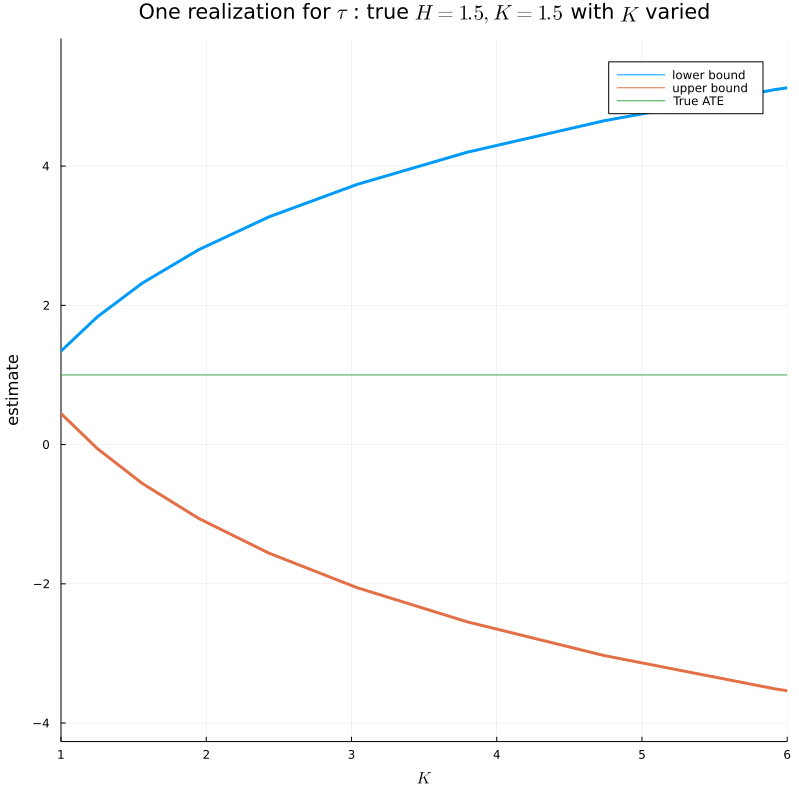
\includegraphics[width=0.6\textwidth]{fig1.png}
        \caption{One realization}
        \label{fig:my_label}
    \end{figure}
    
    \begin{figure}[!htbp]\label{fig:fig2}
        \centering
        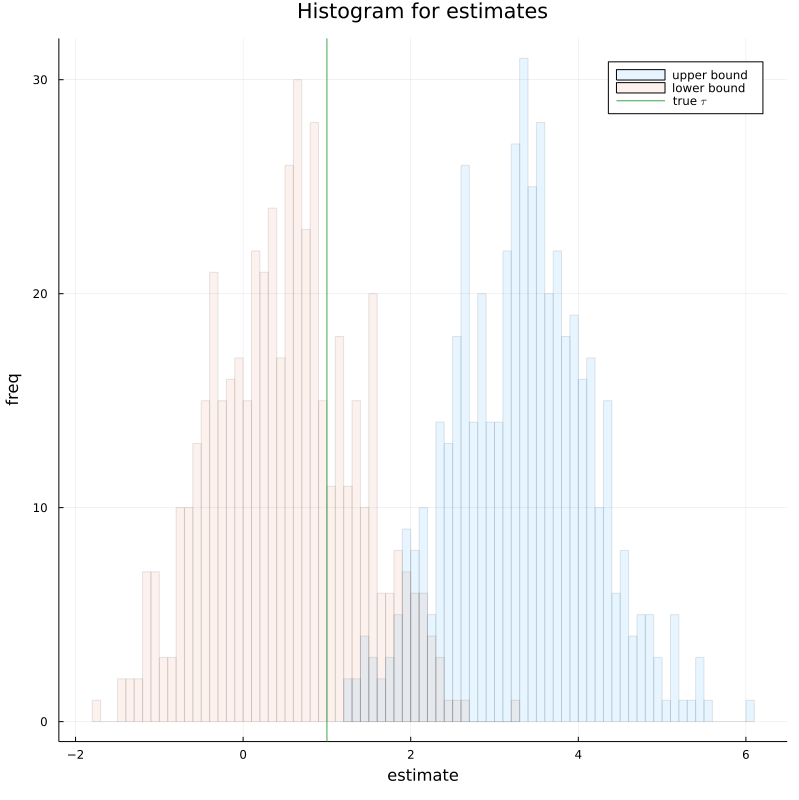
\includegraphics[width = 0.6 \textwidth]{fig2.png}
        \caption{Histogram of Simulated Bounds}
        \label{fig:my_label}
    \end{figure}
    
    I demonstrate the finite sample coverage property of confidence intervals for different $n$ in table 1. Because the true parameter $\tau$ is known from the simulation design, coverage statistics are estimable, and are presented for a number of choices of $n$ varying from 500 to 2000 in Table 1. The main takeaway is that the coverage property is good even in small sample.
    
    \begin{table}
    \begin{threeparttable}
    \caption{Monte Carlo Results: $B = 2000, \tau = 1, K = H = 1$}
        \begin{tabular}{|c|c|c|c|c|c|c|c|}
        \hline $\mathrm{n}$ & $\widehat{\tau}^{-}$ & $\widehat{\sigma}^{-}$ & \text {Std. dev. of } $\widehat{\tau}^{-}$ & $\widehat{\tau}^{+}$ & $\widehat{\sigma}^{+}$ & \text {Std. dev. of } $\widehat{\tau}^{+}$ & \text {Coverage } \\
        \hline 500 & 1.001 & 0.241 & 0.332 & 1.837 & 0.208 & 0.249 & 0.929 \\
        1000 & 0.980 & 0.168 & 0.185 & 1.801 & 0.159 & 0.172 & 0.967 \\
        2000 & 0.985 & 0.122 & 0.132 & 1.784 & 0.117 & 0.126 & 0.965 \\
        \hline
        \end{tabular}
    \begin{tablenotes}
      \small
      \item Coverage statistics from $B = 2000$ simulations generated from a randomly selected linear model with d = 4 observed covariates. The true ATE in the simulation is $\tau = 1$, and unobserved confounding is chosen such that simulation satisfies $K = H = 1.5$. Std. dev. of $\tau^-$ refers to standard deviation between simulation runs (likewise for $\tau^+$. Coverage is for estimated 95\% confidence intervals $(\hat{\tau}^- - 1.96 \hat{\sigma}^-, \hat{\tau}^+ + 1.96 \hat{\sigma}^+)$. These are conservative because the true model cannot simultaneously be upward biased and downward biased. Therefore, we would expect a model under worst-case confounding to converge to 97.5\% coverage.
    \end{tablenotes}
  \end{threeparttable}
  \end{table}
    
    \begin{table}
    \begin{threeparttable}
    \caption{Monte Carlo Results: $B = 2000, \tau = 1, K = H = 1.5$}
        \begin{tabular}{|c|c|c|c|c|c|c|c|}
        \hline $\mathrm{n}$ & $\widehat{\tau}^{-}$ & $\widehat{\sigma}^{-}$ & \text {Std. dev. of } $\widehat{\tau}^{-}$ & $\widehat{\tau}^{+}$ & $\widehat{\sigma}^{+}$ & \text {Std. dev. of } $\widehat{\tau}^{+}$ & \text {Coverage } \\
        \hline 500 & 1.001 & 0.241 & 0.332 & 1.837 & 0.208 & 0.249 & 0.929 \\
        1000 & 0.980 & 0.168 & 0.185 & 1.801 & 0.159 & 0.172 & 0.967 \\
        2000 & 0.985 & 0.122 & 0.132 & 1.784 & 0.117 & 0.126 & 0.965 \\
        \hline
        \end{tabular}
    \begin{tablenotes}
      \small
      \item Coverage statistics from $B = 2000$ simulations generated from a randomly selected linear model with d = 4 observed covariates. The true ATE in the simulation is $\tau = 1$, and unobserved confounding is chosen such that simulation satisfies $K = H = 1.5$. Std. dev. of $\tau^-$ refers to standard deviation between simulation runs (likewise for $\tau^+$. Coverage is for estimated 95\% confidence intervals $(\hat{\tau}^- - 1.96 \hat{\sigma}^-, \hat{\tau}^+ + 1.96 \hat{\sigma}^+)$. These are conservative because the true model cannot simultaneously be upward biased and downward biased. Therefore, we would expect a model under worst-case confounding to converge to 97.5\% coverage.
    \end{tablenotes}
  \end{threeparttable}
  \end{table}
    
	\medskip
	
	\pagebreak
	\nocite{*}
	\printbibliography
	
	\pagebreak
	\appendix
	\section{Proofs}

	
	\duality*
	
	\begin{proof}
		The proof is similar to the one presented in \textcite{yadlowsky2018bounds}. 
		
		First, note that $\mathbb{E}[L(W(1))f(W(1)) \mid D=1]$ is a linear functional of $L(y)$ and thus, a convex functional. Next, the constraint on $L(w)$ are such that the constraint set is convex, so strong duality (see, for example, \textcite{luenberger1997optimization}) holds: by the principle of lagrangian, the original problem can be written as
		$$
		\begin{array}{ll}
		\sup_{\mu} & \inf _{L(w)} \quad \mathbb{E}[L(W(1))f(W(1)) \mid D=1] + \mu(1 -  \mathbb{E}L[W(1)\mid D = 1]) \\
		\text { s.t. }  & L(w) \geq 0, L(w) \leq K L(\tilde{w}) \text { for almost every } w, \tilde{w} \in \mathbb{R}
		\end{array}
		$$
		so the equivalence between the first two problem is established.
		
		The rest follows the same argument as in \textcite{yadlowsky2018bounds}(might include for ease of reading now).
		
		Next, consider the problem of 
		$$
		\begin{array}{ll}
		\inf _{L(w)} & \quad \mathbb{E}[(f(W(1))-\mu) L(Y(1)) \mid D=1]+\mu \\
		\text { s.t. } &\quad L(w) \geq 0, L(w) \leq K L(\tilde{w}) \text { for all } y, \tilde{w} \in \mathbb{R}.
		\end{array}
		$$
		
		For fixed $\mu$, to make the quantity as small as possible, it must be that $L(W(1)) \propto K \Indc(W(1) - \mu \leq 0) + \Indc(W(1) - \mu > 0)$.
		
		Let $L^*(y) = c(K \Indc(f(W(1)) - \mu \leq 0) + \Indc(f(W(1)) - \mu > 0))$, with $c \geq 0$. The problem becomes
		$$
		\begin{array}{ll}
		\sup_{\mu} & \inf _{c \geq 0} \quad c\mathbb{E}\left[(f(W(1))-\mu)_{+}-K(f(W(1))-\mu)_{-} \mid D=1\right] + \mu \\
		\end{array}
		$$
		Suppose $\mathbb{E}\left[(f(W(1))-\mu)_{+}-K(f(W(1))-\mu)_{-} \mid D=1\right] < 0$, the term would be $-\infty$, so the above problem is equal to 
		\begin{equation*}
		\begin{array}{ll}
		\theta_1 \coloneqq & \sup _{\mu}  \mu \\
		& \text { s.t. }  \mathbb{E}\left[(f(W(1))-\mu)_{+}-K(f(W(1))-\mu)_{-} \mid D=1\right] \geq 0.
		\end{array}
		\end{equation*}
		It' s also direct to see that the supremum is attained when the equality holds.
	\end{proof}

	\lb*
	\begin{proof}

		\textbf{(a)} In this case, applying lemma \ref{duality} conditional on $S(1)$ and $G = O$, while taking $f$ as the identity function, for each $s$ we have a lower bound $\theta_1(s)$ for $\Ep[Y(1) \mid S(1) = s, D = 0, G = O]$ given by equation \ref{eq:eq1}. Integration over $S(1) | D = 0, G = O$ gives
		$$\mu^-_1 = \int \theta_1(s) \mathrm{d} P_{S(1) | D = 0, G = O}(s)$$
		which is a valid lower bound on $E[Y(1) \mid D = 0, G = O]$. 
		
		Since sample comparability is maintained, $P_{S(1) \mid G = O}(s) = P_{S(1) \mid G = E}(s) = P_{S(1) \mid D = 1, G = E}(s)$. The total probability formula, on the other hand, gives $$
		P_{S(1) \mid G = O}(s) = P_{S(1) \mid D= 0, G = O}(s) P(D = 0 \mid G = O) +  P_{S(1) \mid D=1, G = O}(s) P(D = 1 \mid G = O),
		$$
		so we can solve for $P_{S(1) \mid D = 0, G = O}(s)$. That gives equation \ref{eq:eq2}.
		
		\textbf{(b)}
		Now consider the more general case where sample comparability assumption might fail. We can no longer point identify $P_{S(1) \mid D = 0, G = O}$ in this case, since $P_{S(1) \mid G = O}$ not necessarily equals $P_{S(1) \mid G = E}$. 
		
		However, note that the quantity $\int \theta_1(s) \mathrm{d} P_{S(1) | D = 0, G = O}(s) = \Ep[\theta_1(S(1)) \mid D = 0, G = O]$ is just another conditional expectation with $\Ep[\theta_1(S(1)) \mid D = 0, G = E]$ point identified. Therefore, viewing $G$ as an assignment in lemma \ref{duality}, we can perform the change of measure again. Here the $f$ in lemma \ref{duality} is $\theta_1$.
		
		Consider the minimization of $\int \theta_1(s) \mathrm{d} P_{S(1) | D = 0, G = O}(s)$, subject to the constraint of $H-$comparability. Note that 
		\begin{align*}
		     \int \theta_1(s) \mathrm{d} P_{S(1) | D = 0, G = O}(s)
		     & = \int \theta_1(s) d \left( \frac{P_{S(1) \mid G = O}(s) - P_{S(1) \mid D = 1, G = O}(s) P(D = 1 \mid G = O)}{P(D = 0 \mid G = O)} \right),
		\end{align*}
		and only non-identified part is $\int \theta_1(s) \mathrm{d} P_{S(1) \mid G = O}$. But then an application of lemma \ref{duality} gives a lower bound for this quantity, as shown in \ref{eq:eq4}. Equation \ref{eq:eq3} then follows.
	\end{proof}
	

    \subsection{Detailed Proof of Consistency and Asymptotic Normality}
	\begin{restatable}{thm}{consistency}
		\label{consistency}
		$\hat{\theta}_{1,s} \overset{p}{\to} \theta_{1,s}$ for all $s \in \{s_1, \ldots, s_k\}$, and $\hat{\zeta}_1 \overset{p}{\to} \zeta_1$. 
	\end{restatable}
	
	\begin{proof}
		For each single $s_k$, the consistency follows from the fact that the following map is strictly increasing and continous in $x$:
		$$\psi_x(y) = (y - x)_+ - K (y - x)_-.$$
		The $Z$-estimator is given by $\Ep_n[\psi_{\hat{\theta}(s)}(Y(1)) \mid S(1) = s, D = 1, G = O] = 0$, which, by Lemma 5.10 in \textcite{van2000asymptotic}, gives an consistent estimator for $\theta_1(s)$.
		
		For $\zeta_1$, define $$\phi_x(y) = (y - x)_+ - H (y - x)_-.$$
		\begin{equation*}
		\mathbb{E}_n\left[(\hat{\theta}_1(S(1))-\hat{\zeta}_1)_{+}-H(\hat{\theta}_1(S(1))-\hat{\zeta}_1)_{-} \mid T=1, G = E\right] = 0
		\end{equation*} 
		can be written as 
		\begin{equation*}
		\mathbb{E}_n\left[ \phi_{\hat{\zeta}_1}(\hat{\theta}_1(S(1)))\mid T=1, G = E\right] = 0.
		\end{equation*}
		Note that $\phi_{x}(y)$ is uniformly continous in each argument when we fix the other one. By continous mapping theorem,
		\begin{equation*}
		\mathbb{E}_n\left[ \phi_{\hat{\zeta}_1}(\theta_1(S(1)))\mid T=1, G = E\right] = \littleop(1).
		\end{equation*}
		Then again by Lemma 5.10 in \textcite{van2000asymptotic}, we have the consistency of $\hat{\zeta}_1$.
	\end{proof}
	
	\begin{restatable}{thm}{asymnorm}
		\label{asymnorm}
		Suppose $P(Y(1) = \theta_{1,s_j} \mid S(1) = s_j, D = 1) = 0$ and $\zeta_1 \neq \theta_{1,s_j}$ for all $k = 1, \cdots, j$. Let $\pi = P(G = E)$. We have
		$$\sqrt{n}(\hat{\theta}_{1,s} - \theta_{1,s}) \overset{d}{\to} N(0,V_s)$$ for all $s \in \{s_1, \ldots, s_k\}$, and $$\sqrt{n}(\hat{\zeta}_1-\zeta_1) \overset{d}{\to} N(0,V_{\zeta}).$$ 
		Here, 
		$$V_s = \frac{\Ep[\psi_{\theta_{1,s}}(Y(1))^2 \mid S(1) = s, D = 1]}{\pi P(S(1)=s, D=1) [K P(Y(1) \leq \theta \mid S(1) = s, D = 1) + P(Y(1) > \theta \mid S(1) = s, D = 1)]^2}$$ and
		$$V_{\zeta} = \frac{\sum_{j=1}^k P(S(1) = s_j \mid T = 1)\phi_{\zeta_1}(\theta_{1,j})^2}{(1-\pi)P(T = 1)[H P(S(1) \leq \zeta_1 \mid T = 1) + P(S(1)  > \zeta_1 \mid T = 1)]^2}.$$
		Moreover, the variance is minimal among all GMM estimator. There are natural plug-in estimators for these variances. 
	\end{restatable}
	
	\begin{proof}
		Let $\pi = \Pr(G = E).$ Without loss of generality, encode $G = O$ as $G = 1$ and $G = E$ as $G = 0$. From the above proof in theorem \ref{consistency}, we can see that for each $\theta_1(s)$, we can establish the corresponding asymptotic variance.
		$$\Ep[\psi_{\theta_1(s)}(Y(1)) \mid S(1) = s, D = 1, G = O] = 0$$ is equivalent with 
		$$\Ep[\Indc(S_i(1) = s) D_iG_i\psi_{\theta_1(s)}(Y_i(1))] = 0.$$
		Let $Z_i = (Y(1), S(1), T, D, G)$. Define $m_{\theta_1(s)}(Z_i) = \Indc(S_i = s, D_i=1) G_i \psi_{\theta(s)}(Y(1)).$ The above moment condition is then $$\Ep[m_{\theta_1(s)}(Z_i)] = 0.$$ 
		Moreover, the moment for $S(1)$ is given by 
		$$\mathbb{E}\left[ T_i(1-G_i)\phi_{\zeta_1}(\theta_1(S_i(1)))\right] = 0.$$
		Rewrite the system of moments as follows:
		\begin{align*}
		\Ep[G\Indc(S(1) = s_1) D \psi_{\theta_{1,1}}(Y(1))] & = 0\\
		& \cdots \\
		\Ep[G\Indc(S(1) = s_k) D \psi_{\theta_{1,k}}(Y(1))] & = 0\\
		\Ep[(1-G) \sum_{j =1}^k \Indc(S(1) = s_j) T \phi_{\zeta_1}(\theta_{1,j})] & = 0
		\end{align*}
		This is a just identified system with noncorrelated moments.
		Let's first focus on the first $k$ equations.
		
		To prove asymptotic normality, I resort to Lemma 5.21 in \textcite{van2000asymptotic}. We need to verify all the conditions needed. The first one is Lipschitz continuity. This follows naturally since $\psi_{\theta}(y)$ is $K-$Lipschitz continuous. The constant function is certainly integrable, so we are done. The second one is differentiability. For the first $k$ equations, $P\psi_{\theta}$ can be shown to be differentiable. Too see this, consider the following simple demonstration: 
		\begin{align*}
		\frac{\partial}{\partial \theta}\Ep[\psi_{\theta}(Y(1))] & = \frac{\partial}{\partial \theta} \Ep[(Y(1) - \theta)_+ - K (Y(1) - \theta)_-].
		\end{align*}
		We have
		$$\frac{\partial}{\partial \theta} \Ep[(Y(1) - \theta)_+] = F_{Y(1)}(\theta) - 1$$
		and 
		$$\frac{\partial}{\partial \theta} \Ep[K(Y(1) - \theta)_-] = K F_{Y(1)}(\theta) $$
		by the absolute continuity of $F_{Y(1)}$.
		
		Applying Lemma 5.21 in \textcite{van2000asymptotic}, we have $\sqrt{n} (\hat{\theta}_1(s) - \theta_1(s)) \overset{d}{\to} N(0, V_s)$ where 
		$$V_s = \frac{\Ep[\psi_{\theta_{1,s}}(Y(1))^2 \mid S(1) = s, D = 1]}{\pi P(S(1)=s, D=1) [K P(Y(1) \leq \theta \mid S(1) = s, D = 1) + P(Y(1) > \theta \mid S(1) = s, D = 1)]^2}$$
		
		Now, for the asymptotic distribution of $\zeta$, the process is essentially similar and $$V_* = \frac{\sum_{j=1}^k P(S(1) = s_j)\phi_{\zeta_1}(\theta_{1,j})^2}{(1-\pi)P(T = 1)[H P(S(1) \leq \zeta_1 \mid T = 1) + P(S(1)  > \zeta_1 \mid T = 1)]^2}.$$
	\end{proof}
	
\end{document}